%!TEX TS-program = xelatex
%!TEX encoding = UTF-8 Unicode
%!TEX root = ../../../LSSN.tex

%------------------------- IMMAGINE TIKZ
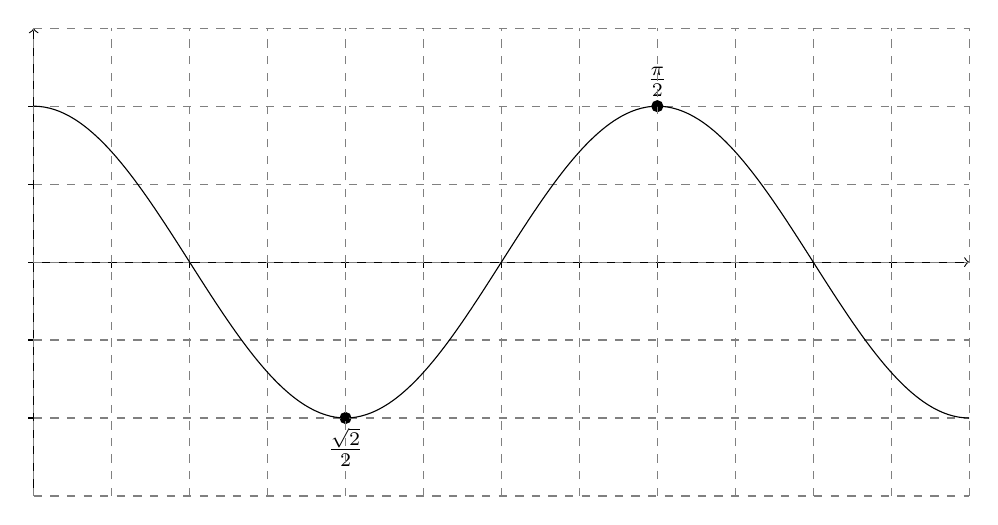
\begin{tikzpicture}[scale=.99]

    \draw[->] (0,-3) -- (0,3);
    \draw[->] (0,0) -- (12,0);
    \foreach \x in {1,2,3,4,5,6,7,8,9,10,11}
        \draw (\x,2pt) -- (\x,-2pt);
    \foreach \y in {-2,-1,0,1,2}
        \draw (2pt,\y) -- (-2pt,\y);

\coordinate (A) at (8,2);
\coordinate (B) at (4,-2);
\filldraw (A) circle (2pt) node[above] {{$\frac{\pi}{2}$}};
\filldraw (B) circle (2pt) node[below] {{{$\frac{\sqrt2}{2}$}}};

   \draw[dashed, gray] (0,-3) grid (12,3);
   %\draw[help lines] (0,-3) grid (12,3);
   \draw (0,2) cos (2,0) sin (4,-2) cos (6,0) sin (8,2) cos (10,0) sin (12,-2);
   %%\draw (0,0) to (12,0);
   \label{sin001}
\end{tikzpicture}
%------------------------- IMMAGINE TIKZ
